\chapter{Tests on Discrete Data}

Data can be discrete for different reasons. On is that you acquired them in a discrete way (e.g. levels in a questionnaires.) Another one is that your paradigm only gives discrete results (e.g. rolling a dice). For the analysis of such data, we can build on the tools that we have already covered in the previous chapters.

\section{Comparing Groups of Ranked Data}

Ordinal data have clear rankings, e.g. "none - little - some - much - very much". However they are not continuous. For the analysis of such \emph{rank ordered data} we can use rank order methods for the analysis:

\begin{description}
  \item[Two groups] When comparing two rank ordered groups, we can use the \emph{Mann-Whitney test} \ref{test:Mann-Whitney}
  \item[Three or more groups]  When comparing two rank ordered groups, we can use the \emph{Kruskal-Wallis test} \ref{test:Kruskal-Wallis}

\end{description}

\section{Logistic Regression}

A more complex question arises when the requirement arises not only to compare two groups, but also to make quantitative predictions for ordinal data. For example, suppose you want to calculate the probability that a patient survives an operation, based on the amount of anesthetic he/she receives. The answer to this question involves statistical modelling, and the tool of \emph{logistic regression}\index{general}{logistic regression}. If more than two ordinal (i.e. naturally ranked) levels are involved, the so-called \emph{ordinal logistic regression}\index{general}{ordinal logistic regression} is used.

\emph{Hypothesis tests} allow you to state quantitative probabilities on the likelihood of a hypothesis. \emph{Linear Regression Modeling} allows you to make predictions and give confidence intervals for output variables that depend linearly on given inputs. But a large class of problems exceeds these requirements. For example, suppose you want to calculate the probability that a patient survives an operation, based on the amount of anesthetic he/she receives, and you want to find out how much anesthetic you can give the patient so that the chance of survival is at least 95\%.

To cover such questions \emph{Generalized Linear Models (GLMs)} have been introduced, which extend the technique of linear regression to a wide range of other problems. A general coverage of GLMs is beyond the goals of this book, and I would like to refer to the excellent book by Dobson \cite{Dobson2008}. While Dobson only gives solutions in \emph{R} and \emph{Stata}, I have made solutions in Python available for most of their problems (\url{https://github.com/thomas-haslwanter/dobson.git}).

In the following chapter I want to cover one commonly used case, \emph{logistic regression}, and its extension to \emph{ordinal logistic regression}. The Python solutions presented should allow the readers to solve similar problems on their own, and should give a brief insight in Generalized Linear Models.

\section{Logistic Regression}\index{general}{Logistic Regression}

So far we have been dealing with linear models, where a linear change on the input leads to a corresponding linear change on the output (Fig. \ref{fig:regression}):

 \begin{equation}\label{eq:linear}
   y = k*x + d + \epsilon
 \end{equation}

However, for many applications this model is not suitable. Suppose we want to calculate the probability that a patient survives an operation, based on the amount of anesthetic he/she receives. This probability is bounded on both ends, since it has to be a value between $0$ and $1$.

We can achieve such a bounded relationship, though, if we don't use the output of Eq. \ref{eq:linear} directly, but wrap it by another function:

\begin{equation}\label{eq:logisticFcn}
  p(x) = \frac{1}{ 1 + e^{ \;\beta x + \alpha } }
\end{equation}

In this model, the variable $\beta$ that describes how quickly the function changes from 1 to 0, and $\alpha$ indicates the location of this change. This function is used frequently, and is called the \emph{logistic function}\index{general}{logistic function}.

\subsection{Example: The Challenger Disaster}

On January 28, 1986, the twenty-fifth flight of the U.S. space shuttle program ended in disaster when one of the rocket boosters of the Shuttle Challenger exploded shortly after lift-off, killing all seven crew members. The presidential commission on the accident concluded that it was caused by the failure of an O-ring in a field joint on the rocket booster, and that this failure was due to a faulty design that made the O-ring unacceptably sensitive to a number of factors including outside temperature. Of the previous 24 flights, data were available on failures of O-rings on 23, (one was lost at sea), and these data were discussed on the evening preceding the Challenger launch, but unfortunately only the data corresponding to the 7 flights on which there was a damage incident were considered important and these were thought to show no obvious trend. The data are shown below:

\begin{figure}[ht]
  \centering
  \includegraphics[width=0.5\textwidth]{../Images/Challenger_ORings.png}\\
  \caption{Failure of O-rings during space shuttle launches, as a function of temperature.}
\end{figure}

To simulate the probability of the O-rings failing, we can use the \emph{logistic function}:

\begin{equation}\label{eq:logisticFcn}
  p(t) = \frac{1}{ 1 + e^{ \;\beta t + \alpha } }
\end{equation}

With a given p-value, the \emph{binomial distribution} (section \ref{sec:binomialDist}) determines the probability mass function for a given number of shuttle launches.

\lstinputlisting[label=py:Logistic,caption=logitShort.py, language=Python]{../Code3/logitShort.py}

\begin{figure}
  \centering
  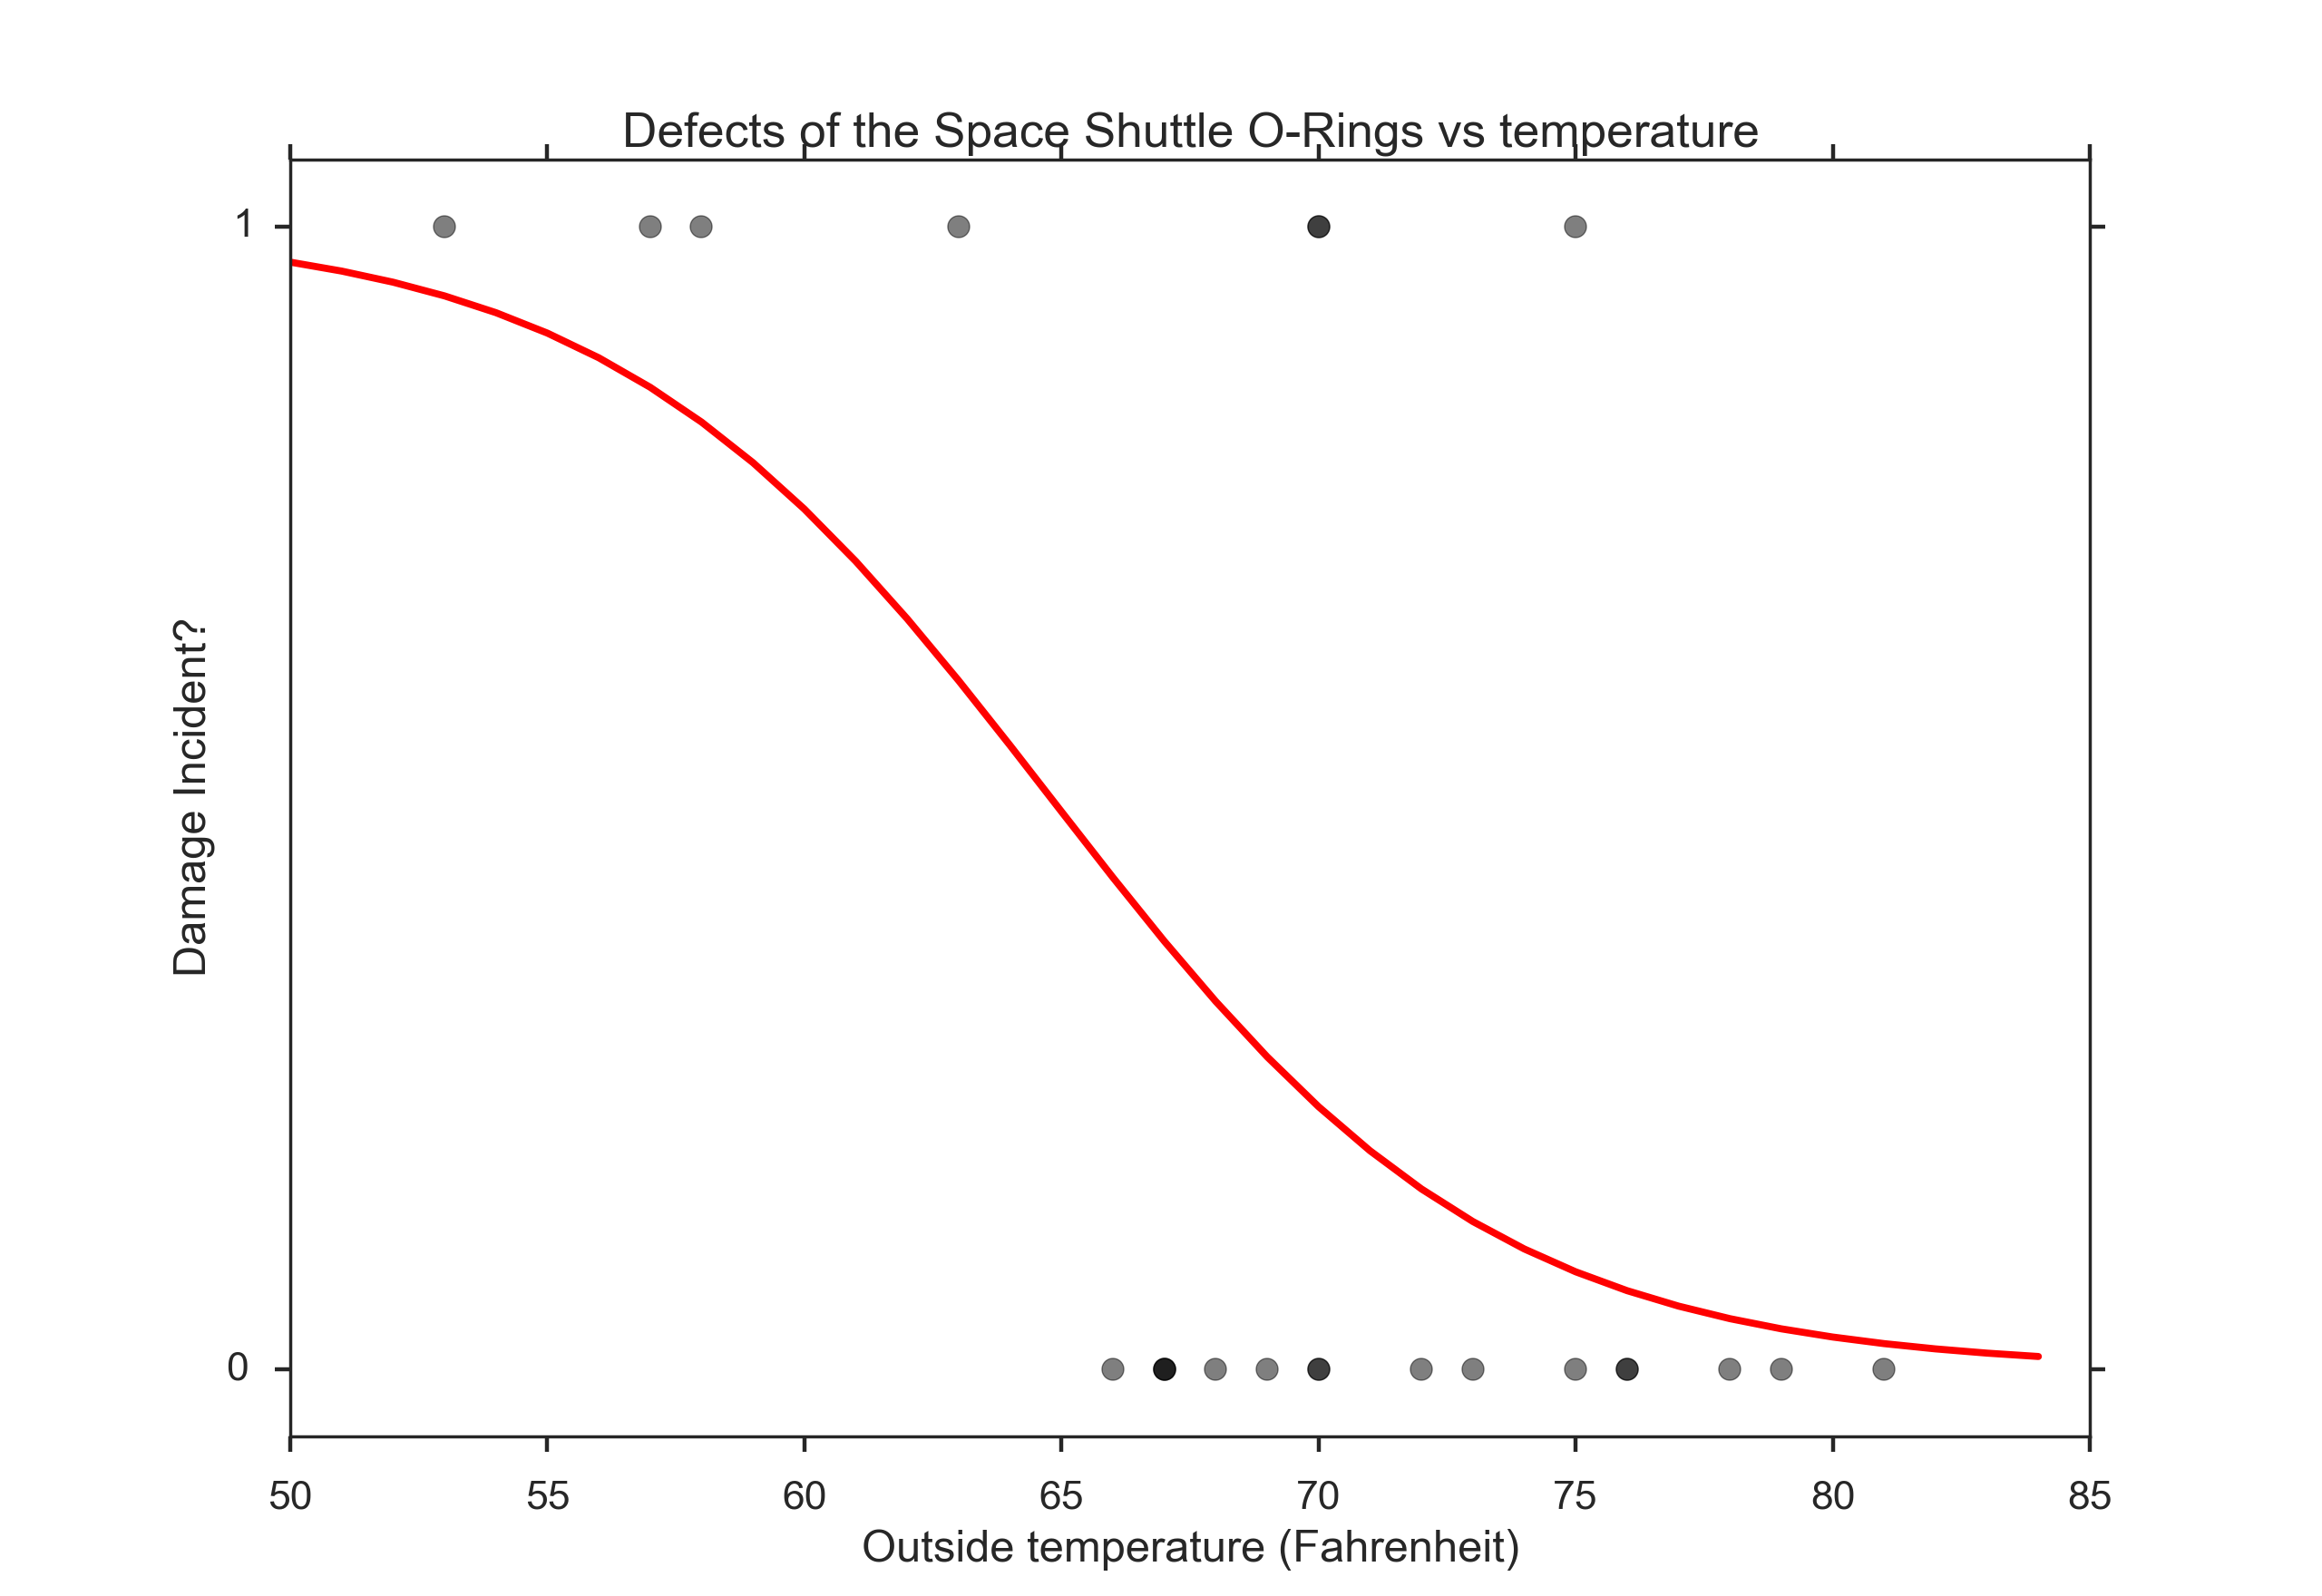
\includegraphics[width=0.75\textwidth]{../Images/ChallengerPlain.png}\\
  \caption{Probability for O-ring failure.}
  \label{fig:challengerPlain}
\end{figure}

\PyImg "logit.py" (p \pageref{py:logit}) shows the full code for Fig. \ref{fig:challengerPlain}.
\index{python}{modeling}

\vspace{5 mm}

To summarize, we have three elements in our model

\begin{enumerate}
  \item A probability distribution, which determines the probability of the outcome for a given trial (here the binomial distribution).
  \item A linear model that relates the co-variates (here the temperature) to the variates (the failure/success of an O-ring).
  \item A \emph{link-function}\index{general}{link-function} that wraps the linear model to produce the parameter for the probability distribution.
\end{enumerate}

%Similarly, a model that predicts a probability of making a yes/no choice (a Bernoulli variable) is even less suitable as a linear-response model, since probabilities are bounded on both ends (they must be between 0 and 1). Imagine, for example, a model that predicts the likelihood of a given person going to the beach as a function of temperature. A reasonable model might predict, for example, that a change in 10 degrees makes a person two times more or less likely to go to the beach. But what does "twice as likely" mean in terms of a probability? It cannot literally mean to double the probability value (e.g. 50% becomes 100%, 75% becomes 150%, etc.). Rather, it is the odds that are doubling: from 2:1 odds, to 4:1 odds, to 8:1 odds, etc. Such a model is a log-odds model.

\section{Generalized Linear Models}\index{general}{Generalized Linear Models}

The example above is an example of a \emph{Generalized Linear Models (GLMS)}, a powerful tool for the analysis of wide range of statistical models. Here I will only describe the general principles. For details I refer to the excellent book by \cite{Dobson2008}.

A GLM consists of three elements:

\begin{enumerate}
  \item A probability distribution from the \emph{exponential family}\index{general}{distributions!exponential family}.
  \item A linear predictor $\eta = X \cdot \beta$ .
  \item A link function $g$ such that $E(Y) = \mu = g^{-1}(\eta)$.
\end{enumerate}

\subsection{Exponential Family of Distributions}

The exponential family is a set of probability distributions of a certain form, specified below. This special form is chosen for mathematical convenience, on account of some useful algebraic properties, as well as for generality, as exponential families are in a sense very natural sets of distributions to consider. The exponential families include many of the most common distributions, including the normal, exponential, chi-squared, Bernoulli, Poisson distribution and many others. (A common distribution that is not from the exponential family is the T-distribution.)

In mathematical terms, an distribution from the exponential family has the general form

\begin{equation}\label{eq:exponentialFamily}
  f_X(x|\theta) = h(x) g(\theta) \exp \left ( \eta(\theta) \cdot T(x) \right )
\end{equation}

where $T(x), h(x), g(\theta), \eta(\theta), and A(\theta)$ are known functions.

\subsection{Linear Predictor and Link Function}

The linear predictor for GLM is the same as the one used for \emph{linear models}. The resulting terminology is unfortunately fairly confusing:

\begin{description}
  \item[General Linear Models] are models of the form $y=X\beta+ \epsilon$, where $\epsilon$ is normally distributed (see Chapter \ref{chapter:models}).
  \item[Generalized Linear Models] encompass a much wider class of models, including all distributions from the exponential family \emph{and} a link function.
\end{description}

The \emph{link function} is an arbitrary function, with the only requirements that it is continuous and invertable.

\section{Ordinal Logistic Regression}\index{general}{Ordinal Logistic Regression}

\begin{eqnarray*}{rl}
    log (P(Y\ge 1|X) &=& 1/[1 + exp(-(\alpha_1 + B_1 X_1 + ….+ B_{n-1} X_{n-1}))]\\
    log (P(Y\ge 2|X) &=& 1/[1+exp(-(\alpha_2 + B_1 X_1 + ….+ B_{n-1} X_{n-1}))]\\
    …. &=& …. \\
    log (P(Y \ge m-2|X) &=& 1/ [1 + exp[-( \alpha_{m-2}+ B_1 X_1 + ….+ B_{n-1} X_{n-1}))]\\
    log (P(Y \ge m-1|X) &=& 1/ [1 + exp(\alpha_{m-1}+ B_1 X_1 + ….+ B_{n-1} X_{n-1}))]\\
\end{eqnarray*}

The probability that $$Y = k$$, is then given by $$P(Y = k|X) = P(Y\ge k) -P(Y\ge k+1)$$. Of course we have $$(Y = m-1|X) = P(Y\ge m-1|X)$$ at the boundary with $$P(Y\ge 0|X) = 1.0$$.

The likelihood function is given by the following formula:

$$L=\prod_{i= 0}^{N-1} \prod_{k=0}^{m-1 }P(Y= j|X)^{\delta_k^j}$$

where $$\delta_k^j= 1$$ if $$k = j$$, otherwise it is zero. The coefficients are obtained by maximizing L using an optimizer. It is more convenient to work with logarithms and the logarithm is then called the log likelihood function. Most statistical softwares will multiply the result by -2 so that a minimizer can be used to optimize the log likelihood value.

Here is our Python module for performing ordinal logistic regression. It currently focuses on determining the coefficients of the model specified above. 